\documentclass[paper=a4, fontsize=10pt]{scrartcl}
\usepackage[bottom=0.8in, left=0.5in, right=0.5in, top=0.8in, foot=0.4in]{geometry}
\usepackage{layouts}

\usepackage[usenames,dvipsnames,x11names]{xcolor}

\usepackage[T1]{fontenc}
\usepackage{fourier}
\usepackage[english]{babel}
\usepackage{amsmath,amsfonts,amsthm}

\usepackage{sectsty}
\allsectionsfont{\centering \normalfont\scshape}

\usepackage{acronym}
\usepackage{booktabs}
\usepackage{caption}
\usepackage{fancyhdr}
\usepackage{float}
\usepackage{graphicx}
\usepackage[htt]{hyphenat}
\usepackage{lastpage}
\usepackage{listings}
\usepackage{longtable}
\usepackage{minted}
\usepackage{multicol}
\usepackage{multirow}

\pagestyle{fancyplain}
\fancyhead{}
\fancyfoot[L]{}
\fancyfoot[C]{\thepage~of~2}
\renewcommand{\headrulewidth}{0pt}
\renewcommand{\footrulewidth}{0pt}
\setlength{\headheight}{13.6pt}

\newcommand{\horrule}[1]{\rule{\linewidth}{#1}}

\usepackage{tikz}
\usetikzlibrary{plotmarks}
\usepackage{pgfplots, pgfplotstable}
\pgfplotsset{compat=1.5}
\usepgfplotslibrary{colorbrewer}
\usepgfplotslibrary{fillbetween}
\usepgfplotslibrary{groupplots}

% http://tex.stackexchange.com/questions/67895/is-there-an-easy-way-of-using-line-thickness-as-error-indicator-in-a-plot

% Takes six arguments: data table name, x column, y column, error column,
% color and error bar opacity.
% ---
% Creates invisible plots for the upper and lower boundaries of the error,
% and names them. Then uses fill between to fill between the named upper and
% lower error boundaries. All these plots are forgotten so that they are not
% included in the legend. Finally, plots the y column above the error band.
\newcommand{\errorband}[6]{
\pgfplotstableread{#1}\datatable
  \addplot [name path=pluserror,draw=none,no markers,forget plot]
    table [x={#2},y expr=\thisrow{#3}+\thisrow{#4}] {\datatable};

  \addplot [name path=minuserror,draw=none,no markers,forget plot]
    table [x={#2},y expr=\thisrow{#3}-\thisrow{#4}] {\datatable};

  \addplot [forget plot,fill=#5,opacity=#6]
    fill between[on layer={},of=pluserror and minuserror];

  \addplot [#5,thick,no markers]
    table [x={#2},y={#3}] {\datatable};
}

\title{
\vspace{-1cm}
\normalfont \normalsize
\textsc{Norwegian University of Science and Technology\\IT3708 -- Bio-Inspired Artificial Intelligence}
\horrule{0.5pt} \\[0cm]
\huge Project 1:\\ Supervised and Reinforcement Learning of\\Neural Agent Controllers\\[-0.3cm]
\horrule{2pt} \\[0.1cm]
}

\author{Per Magnus Veierland\\permve@stud.ntnu.no}

\date{\normalsize\today}

\begin{document}

\maketitle

\begin{multicols}{2}

\section*{Implementation and Baseline}

The assignment program is a single file \texttt{flatland.py} written using the Python programming language with the NumPy library for computation. PyQt bindings are used to render vector graphics to PDF. The visualization uses an \textsc{X} to mark the agent starting point, and an increasing line thickness to indicate the direction of movement. The most important classes are the \texttt{BaselineAgent} and \texttt{LearningAgent}. They both implement the method \texttt{act} which takes a \texttt{percepts} parameter and returns an \texttt{Action}. The \texttt{percepts} parameter is a $(3,S)$ N-dimensional array, where the first dimension is the direction, and the second is the sensor range ($S$). The \texttt{LearningAgent} also provides the methods \texttt{evaluate}; which takes a \texttt{percepts} parameter and returns a tuple of one-hot encoded inputs and the neural network outputs, and the method \texttt{update\_weights}; which updates the network weights given a learning rate, a delta, and network inputs. \texttt{SupervisedAgent} and \texttt{ReinforcementAgent} both inherit from \texttt{LearningAgent} and implement separate \texttt{train} methods.

{
\vspace{0.3cm}
\centering
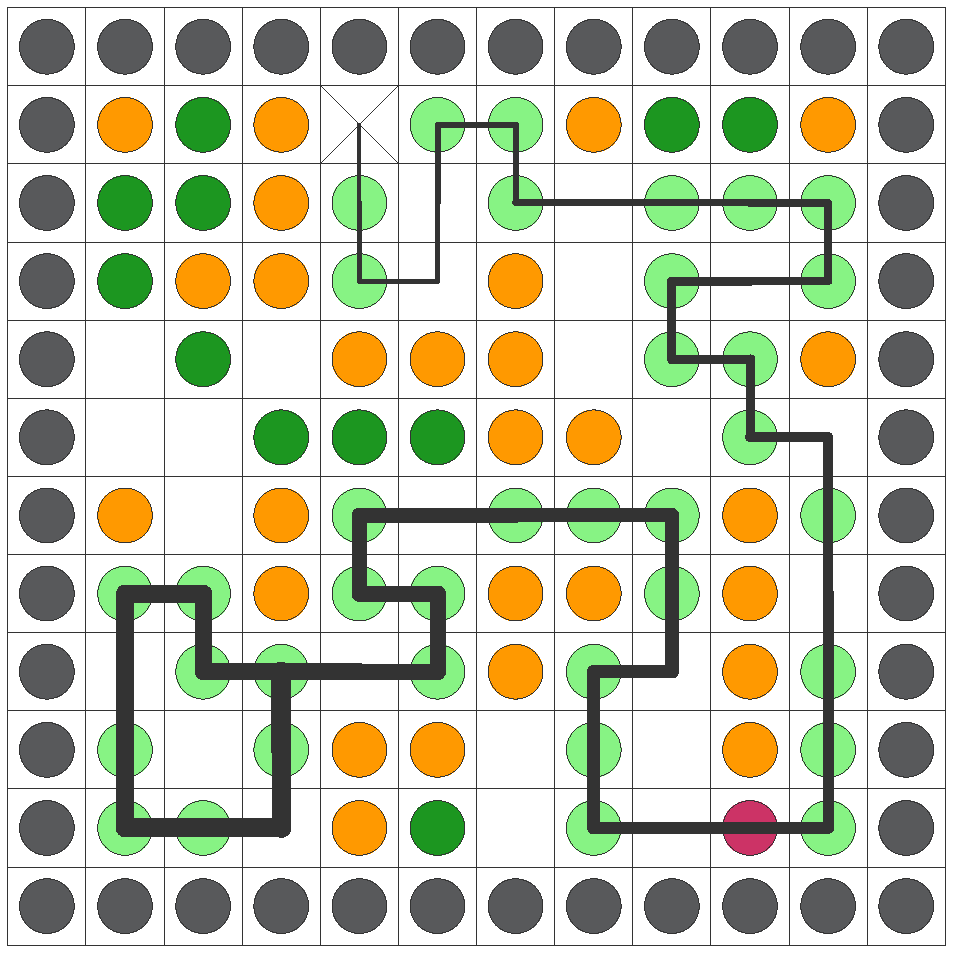
\includegraphics[scale=0.2]{../data/render-baseline.pdf}
\captionof{figure}{Flatland visualization of baseline agent}
\label{figure:flatland_baseline}
\vspace{0.3cm}
}

The baseline agent behavior is to always move towards food. If there is no neighboring food, it will move towards an empty location. If there are no empty locations it will move towards poison. Given how the world is defined the baseline agent will never need to move into walls. If there are more than one possible destination of the same kind, it will prefer moving forward, otherwise left, otherwise right, accordingly.

The mean score achieved by the baseline agent is $20.2$ averaged over 1~million~trials.

\vspace{-0.3cm}
\section*{Supervised Learning Agent}

The computation of the delta term as part of the \textit{Widroff-Hoff rule} is shown in Figure~\ref{fig:code_delta_supervised}. The \textit{CorrectChoice} is a \textit{one-hot encoded} vector where the index of the target action is set to 1. To make the softmax computation numerically stable the reformulation described in Equation~\ref{eq:softmax} is used, with ${\log C = -\max_k y_k}$, such that the greatest exponent factor is 0.

\begin{equation}
\frac{e^{y_j}}{\sum_k e^{y_k}} = \frac{C \cdot e^{y_j}}{C \cdot \sum_k e^{y_k}} = \frac{e^{y_j + \log C}}{\sum_k e^{y_k + \log C}}
\label{eq:softmax}
\end{equation}

{
\footnotesize
\begin{minted}[mathescape,
               linenos,
               numbersep=5pt,
               frame=lines,
               framesep=2mm,
               xleftmargin=3mm,
               xrightmargin=3mm]{python}
def train(self, percepts, target_action, learning_rate):
  inputs, outputs = self.evaluate(percepts)
  outputs        -= np.max(outputs)
  softmax         = np.exp(outputs) / np.sum(np.exp(outputs))
  correct_choice  = encode_int_as_one_hot(target_action, 3)
  delta           = correct_choice - softmax
  self.update_weights(learning_rate, delta, inputs)
\end{minted}
\vspace*{-3mm}
\captionof{figure}{The \texttt{train} method of \texttt{SupervisedAgent}}
\label{fig:code_delta_supervised}
}

\vspace{-0.3cm}
\section*{Reinforcement Learning Agent}

The computation of the delta term for the agent trained using reinforcement learning is shown in Figure~\ref{fig:code_delta_reinforcement}. The network is evaluated using the \texttt{percepts} from both before and after the action is applied. The current \textit{Q-value} is the maximum network output given the pre-action \texttt{percepts}, and the next \textit{Q-value} is the maximum network output given the post-action \texttt{percepts}. Since only the neuron corresponding to the taken action is updated, the scalar ${r + \gamma \max_{a'} Q(s', a') - Q(s, a)}$ is multiplied with a \textit{one-hot encoded} action vector.

\vspace{-0.3cm}
\section*{Analysis}

A clear structure can be seen in the reinforcement agent weights (Table~\ref{table:weights}), where for each direction the four weights linked to the input to the output is ordered in the same way such that the ``food weight'' is the strongest, then the ``empty weight'', then the ``poison weight'', then the ``wall weight''.

The performance of the agent trained using supervised learning closely matches the performance of the baseline agent. This was expected as the baseline behavior is a simple function of preferring food over empty areas, empty areas over poison, and poison over walls. It is also expected that the supervised agent would not surpass the baseline agent since it should learn the baseline agent function. When comparing the reinforcement agent with sensor range~1 to the baseline agent it performs slightly, but distinctly better. This was unexpected as the baseline agent was designed to be optimal.

To understand why the reinforcement agent performs slightly better the scenarios are looked at more closely. With a sensor range of~1 there are 64~possible inputs scenarios, out of which 44~are obvious (e.g.~\textsc{F/W/W}), 6~are left/right ambiguous (e.g.~\textsc{F/W/F}), 6~are sideways/forwards ambiguous (e.g.~\textsc{F/F/O}), 4~are left/forwards/right ambiguous (e.g.~\textsc{F/F/F}), and 4~are non-obvious since they involve a wall on a side and food or an empty area (e.g.~\textsc{W/F/O}. If the behavior of the baseline agent is adjusted such that in scenario \#5 it moves to the side instead of forwards, it ends up performing as good as the reinforcement trained agents, with a score of~$20.8$ when averaged over 1~million~trials. This is an improvement as moving away from the wall increases the probability of avoiding poison. Any slight remaining discrepancy between the reinforcement agent and baseline agent scores is hypothesized to be caused by the reinforcement agent not moving in the same direction for all left/right ambiguous situations, but balancing between both directions for different scenarios.

An agent trained using reinforcement learning and a sensor range of~3 expectedly performs significantly better than the other agents as it is able to exploit more information, e.g. preferring a direction which has two food entities in a row, and avoiding poison or walls which are more than one move away.

{
\footnotesize
\begin{minted}[mathescape,
               linenos,
               numbersep=5pt,
               frame=lines,
               framesep=2mm,
               xleftmargin=3mm,
               xrightmargin=3mm]{python}
def train(self, percepts, percepts_next, learning_rate,
          discount_factor, reward):
  inputs, outputs = self.evaluate(percepts)
  action = np.argmax(outputs)
  q_current = outputs[action]
  q_next = np.amax(self.evaluate(percepts_next)[1])
  delta  = (encode_int_as_one_hot(action, 3) *
    (reward + discount_factor * q_next - q_current))
  self.update_weights(learning_rate, delta, inputs)
\end{minted}
\vspace*{-3mm}
\captionof{figure}{The \texttt{train} method of \texttt{ReinforcementAgent}}
\label{fig:code_delta_reinforcement}
}

\end{multicols}

\begin{figure}[H]
\vspace{-0.5cm}
\centering
\begin{tikzpicture}
\begin{groupplot}[group style={group size=3 by 1, horizontal sep=1.2cm, vertical sep=2cm}]
\nextgroupplot[%
title={Supervised ($S=1$)},
title style={yshift=-1ex},
width=4cm,
height=4cm,
scale only axis,
every x tick label/.append style={font=\scriptsize\color{gray!80!black}},
xmin=1, xmax=30,
xlabel={Training Round},
xlabel style={yshift=0.5ex},
xmajorgrids,
xminorgrids,
every y tick label/.append style={font=\scriptsize\color{gray!80!black}},
ymin=0, ymax=30,
ylabel={Score},
ylabel style={yshift=-0.5ex},
ymajorgrids,
yminorgrids
]
\errorband{../data/learning-curve-supervised-1-sensor-range-30-training-rounds-100-size-30-repetitions.txt}{0}{1}{2}{Cyan}{0.4}
\addplot[mark=none, Magenta, very thick] coordinates {(0,20.2) (30,20.2)};

\nextgroupplot[%
title={Reinforcement ($S=1$)},
title style={yshift=-1ex},
width=4cm,
height=4cm,
scale only axis,
every x tick label/.append style={font=\scriptsize\color{gray!80!black}},
xmin=1, xmax=30,
xlabel={Training Round},
xlabel style={yshift=0.5ex},
xmajorgrids,
xminorgrids,
every y tick label/.append style={font=\scriptsize\color{gray!80!black}},
ymin=0, ymax=30,
ylabel={Score},
ylabel style={yshift=-0.5ex},
ymajorgrids,
yminorgrids
]
\errorband{../data/learning-curve-reinforcement-1-sensor-range-30-training-rounds-100-size-30-repetitions.txt}{0}{1}{2}{Cyan}{0.4}
\addplot[mark=none, Magenta, very thick] coordinates {(0,20.2) (30,20.2)};

\nextgroupplot[%
title={Reinforcement ($S=3$)},
title style={yshift=-1ex},
width=4cm,
height=4cm,
scale only axis,
every x tick label/.append style={font=\scriptsize\color{gray!80!black}},
xmin=1, xmax=30,
xlabel={Training Round},
xlabel style={yshift=0.5ex},
xmajorgrids,
xminorgrids,
every y tick label/.append style={font=\scriptsize\color{gray!80!black}},
ymin=0, ymax=30,
ylabel={Score},
ylabel style={yshift=-0.5ex},
ymajorgrids,
yminorgrids]
\errorband{../data/learning-curve-reinforcement-3-sensor-range-30-training-rounds-100-size-30-repetitions.txt}{0}{1}{2}{Cyan}{0.4}
\addplot[mark=none, Magenta, very thick] coordinates {(0,20.2) (30,20.2)};
\end{groupplot}
\end{tikzpicture}
\vspace{-0.2cm}
\captionsetup{justification=centering,indention=-1.2cm}
\caption{\small{}Agent scores showing gradual learning. Each training round consists of 100~random Flatland worlds. The dark blue lines show the mean across 30 repetitions and the light blue shows the standard deviation. The thick magenta line shows the baseline agent score ($20.2$).\\A learning rate $\alpha = 0.01$ and discount factor $\gamma = 0.9$ is used for all experiments.}
\label{fig:learning_plots}
\vspace{-0.2cm}
\end{figure}

\begin{table}
\centering
\footnotesize
\begin{tabular}{*{13}{c@{\hskip 1.8mm}}}
\toprule
\textsc{Action} & \textsc{LE} & \textsc{LW} & \textsc{LF} & \textsc{LP} & \textsc{FE} & \textsc{FW} & \textsc{FF} & \textsc{FP} & \textsc{RE} & \textsc{RW} & \textsc{RF} & \textsc{RP} \\
\midrule
\textsc{Left} & \textsc{2.27238} & \textsc{-1.99947} & \textsc{3.55820} & \textsc{-1.56634} & \textsc{0.74275} & \textsc{0.06020} & \textsc{0.65737} & \textsc{0.80553} & \textsc{0.45891} & \textsc{0.59558} & \textsc{0.53390} & \textsc{0.67514} \\
\textsc{Forward} & \textsc{0.59295} & \textsc{0.32543} & \textsc{0.56372} & \textsc{0.66674} & \textsc{2.55852} & \textsc{-2.98390} & \textsc{3.89967} & \textsc{-1.32605} & \textsc{0.68196} & \textsc{0.03736} & \textsc{0.65998} & \textsc{0.77091} \\
\textsc{Right} & \textsc{0.50691} & \textsc{0.67649} & \textsc{0.26464} & \textsc{0.51774} & \textsc{0.50082} & \textsc{0.35558} & \textsc{0.41975} & \textsc{0.68855} & \textsc{2.34135} & \textsc{-2.97435} & \textsc{3.87039} & \textsc{-1.27376} \\
\bottomrule
\end{tabular}
\vspace{-0.2cm}
\caption{Weights for agent trained using reinforcement learning with 30 training rounds of 100~Flatland worlds each ($S=1$)}
\vspace{-0.2cm}
\label{table:weights}
\end{table}

\begin{table}
\centering
\footnotesize
\begin{tabular}{*{8}{c@{\hskip 1.8mm}}p{8cm}}
\toprule
\multirow{2}{*}{\textsc{Scenario}} & \multicolumn{3}{c}{\textsc{Network Inputs}} & \multicolumn{3}{c}{\textsc{Network Outputs}} & \multirow{2}{*}{\textsc{Action}} & \multicolumn{1}{c}{\multirow{2}{*}{\textsc{Description}}} \\
~ & \textsc{Left} & \textsc{Forward} & \textsc{Right} & \textsc{Left} & \textsc{Forward} & \textsc{Right} & ~ & ~ \\
\midrule
1 & \textsc{Wall}  & \textsc{Poison} & \textsc{Food}  & $-0.66004$ & $-0.34063$ & $ 5.23544$ & \textsc{Right}   & The network expectedly shows the least preference for the wall, higher preference for the poison, and a greatly higher preference for the food. \\
2 & \textsc{Wall}  & \textsc{Poison} & \textsc{Wall}  & $-0.59836$ & $-0.96325$ & $-1.60930$ & \textsc{Left}    & This is a scenario never encountered during training, and the agent makes a move towards a wall when it should have moved towards poison. \\
3 & \textsc{Empty} & \textsc{Empty}  & \textsc{Wall}  & $ 3.61071$ & $ 3.18884$ & $-1.96661$ & \textsc{Left}    & In this scenario, the agent moves away from the wall instead of moving forward. This is a better action as it increases the probability of avoiding poison in the next turn. \\
4 & \textsc{Wall}  & \textsc{Empty}  & \textsc{Empty} & $-0.79781$ & $ 3.56591$ & $ 3.51867$ & \textsc{Forward} & This scenario mirrors scenario \#3, however the agent moves forward instead of to the side. It can be seen that the two action outputs are very similar, and this would likely be corrected with further training. \\
5 & \textsc{Wall}  & \textsc{Food}   & \textsc{Food}  & $-0.80820$ & $ 4.88509$ & $ 4.96663$ & \textsc{Right}   & In this scenario, the agent moves away from the wall into the food instead of moving forward into the food. \\
\bottomrule
\end{tabular}
\vspace{-0.2cm}
\caption{Selected scenarios illustrating agent behavior resulting from reinforcement learning ($S=1$)}
\vspace{-0.4cm}
\label{table:weights}
\end{table}

\end{document}
